% begin module cycloid-def
\begin{frame}
\frametitle{The Cycloid}
\ \only<handout:0| 1>{%
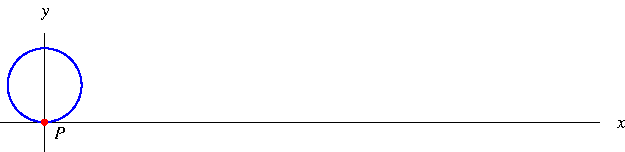
\includegraphics[width=12cm]{parametric-curves/pictures/11-01-cycloida.pdf}%
}%
\only<handout:0| 2>{%
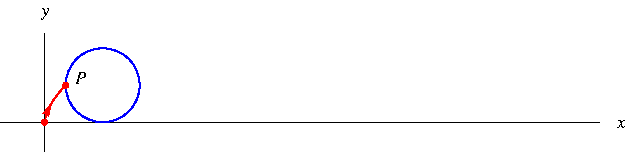
\includegraphics[width=12cm]{parametric-curves/pictures/11-01-cycloidb.pdf}%
}%
\only<handout:0| 3>{%
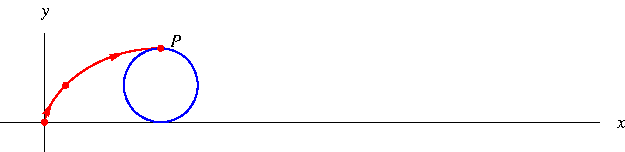
\includegraphics[width=12cm]{parametric-curves/pictures/11-01-cycloidc.pdf}%
}%
\only<handout:0| 4>{%
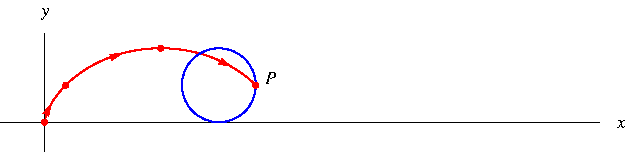
\includegraphics[width=12cm]{parametric-curves/pictures/11-01-cycloidd.pdf}%
}%
\only<handout:0| 5>{%
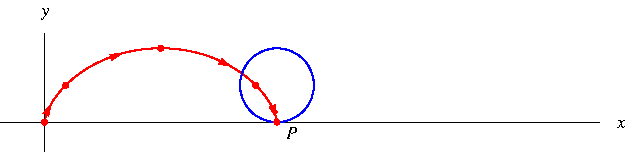
\includegraphics[width=12cm]{parametric-curves/pictures/11-01-cycloide.pdf}%
}%
\only<handout:0| 6>{%
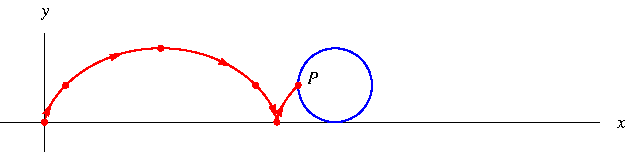
\includegraphics[width=12cm]{parametric-curves/pictures/11-01-cycloidf.pdf}%
}%
\only<handout:0| 7>{%
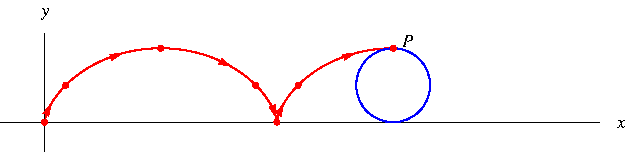
\includegraphics[width=12cm]{parametric-curves/pictures/11-01-cycloidg.pdf}%
}%
\only<8>{%
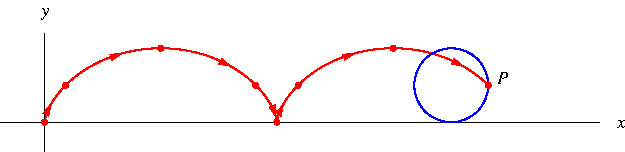
\includegraphics[width=12cm]{parametric-curves/pictures/11-01-cycloidh.pdf}%
}%
\only<handout:0| 9>{%
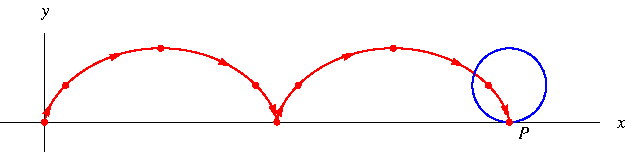
\includegraphics[width=12cm]{parametric-curves/pictures/11-01-cycloidi.pdf}%
}%
\only<handout:0| 10->{%
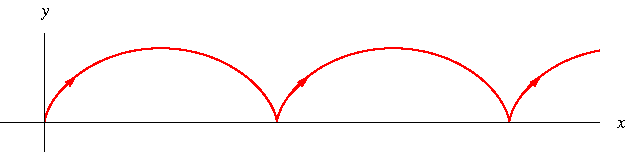
\includegraphics[width=12cm]{parametric-curves/pictures/11-01-cycloidj.pdf}%
}%
\begin{definition}[Cycloid]
The curve traced out by a point $P$ on the circumference of a circle as the circle rolls along a straight line is called a cycloid.
\end{definition}
\end{frame}
% end module cycloid-def
